\documentclass{standalone}
\usepackage{graphicx}	
\usepackage{amssymb, amsmath}
\usepackage{color}

\usepackage{tikz}
\usetikzlibrary{intersections, backgrounds, math, decorations.pathreplacing}
\usepackage{pgfmath}

\definecolor{light}{RGB}{220, 188, 188}
\definecolor{mid}{RGB}{185, 124, 124}
\definecolor{dark}{RGB}{143, 39, 39}
\definecolor{highlight}{RGB}{180, 31, 180}
\definecolor{lightteal}{RGB}{186, 219, 219}
\definecolor{midteal}{RGB}{124, 186, 186}
\definecolor{darkteal}{RGB}{38, 142, 142}
\definecolor{darkerteal}{RGB}{0, 124, 124}
\definecolor{gray10}{gray}{0.1}
\definecolor{gray20}{gray}{0.2}
\definecolor{gray30}{gray}{0.3}
\definecolor{gray40}{gray}{0.4}
\definecolor{gray60}{gray}{0.6}
\definecolor{gray70}{gray}{0.7}
\definecolor{gray80}{gray}{0.8}
\definecolor{gray90}{gray}{0.9}
\definecolor{gray95}{gray}{0.95}

\begin{document}

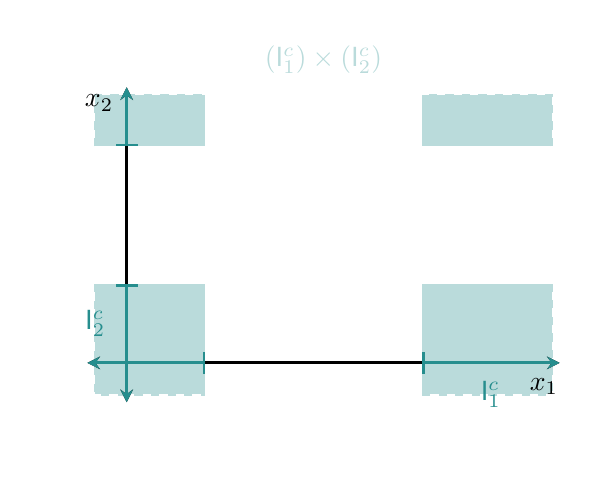
\begin{tikzpicture}[scale=1.0]

  \pgfmathsetmacro{\xa}{-1.5};
  \pgfmathsetmacro{\xb}{1.25};
  \pgfmathsetmacro{\ya}{-0.5};
  \pgfmathsetmacro{\yb}{1.25};
  
  \draw[white] (-3.75, -2.75) rectangle (3.25, 2.75);
  
  \fill[lightteal] (-2.9, -1.9) rectangle (\xa, \ya);
  \draw[lightteal, dashed, line width=1] (-2.9, \ya) -- (-2.9, -1.9) -- (\xa, -1.9);

  \fill[lightteal] (\xb, -1.9) rectangle (2.9, \ya);
  \draw[lightteal, dashed, line width=1] (\xb, -1.9) -- (2.9, -1.9) -- (2.9, \ya);
  
  \fill[lightteal,] (\xb, \yb) rectangle (2.9, 1.9);
  \draw[lightteal, dashed, line width=1] (2.9, \yb) -- (2.9, 1.9) -- (\xb, 1.9);
  
  \fill[lightteal,] (\xa, \yb) rectangle (-2.9, 1.9);
  \draw[lightteal, dashed, line width=1] (-2.9, \yb) -- (-2.9, 1.9) -- (\xa, 1.9);
  
  \draw [<->, >=stealth, line width=1] (-2.5, -2) -- +(0, 4);
  \draw [<->, >=stealth, line width=1] (-3, -1.5) -- +(6, 0);
  
  \node at (2.8, -1.8) { $x_{1}$ };
  \node at (-2.85, 1.8) { $x_{2}$ };
  
  \draw[<-|, >=stealth, darkteal, line width=1] (-3, -1.5) -- (\xa, -1.5);
  \draw[|->, >=stealth, darkteal, line width=1] (\xb, -1.5) -- (3, -1.5);
  \node[darkteal] at ( { 0.5 * ( \xb + 3) }, -1.9) { $\mathsf{I}_{1}^{c}$ };
 
  \draw[<-|, , >=stealth, darkteal, line width=1] (-2.5, -2) -- (-2.5, \ya);
  \draw[|->, , >=stealth, darkteal, line width=1] (-2.5, \yb) -- (-2.5, 2);
  \node[darkteal] at ( -2.9, { 0.5 * ( \ya - 1.5) } ) { $\mathsf{I}_{2}^{c}$ };
  
  \node[lightteal] at (0, 2.35) { 
    $( \mathsf{I}_{1}^{c} ) \times ( \mathsf{I}_{2}^{c} )$ 
  };

\end{tikzpicture}

\end{document}  